\documentclass[a4paper,11pt]{article}

% --- Encodage et Langue ---
\usepackage[utf8]{inputenc}
\usepackage[T1]{fontenc}
\usepackage[french]{babel}

% --- Mise en page et Typographie ---
\usepackage{geometry}
\geometry{margin=2.5cm, headheight=15pt}
\usepackage{microtype}
\usepackage{lmodern}

% --- En-têtes et pieds de page ---
\usepackage{fancyhdr}
\pagestyle{fancy}
\fancyhf{}
\renewcommand{\headrulewidth}{0pt}
\renewcommand{\footrulewidth}{0.4pt}
\fancyfoot[L]{\small\textcolor{primary}{\textit{Copyrights Jean-Christophe Le Lann -- Électronique Numérique}}}
\fancyfoot[R]{\small\textcolor{primary}{\thepage}}

% --- Mathématiques ---
\usepackage{amsmath, amssymb}

% --- Images et Sous-figures ---
\usepackage{graphicx}
\usepackage{float}
%\usepackage{subcaption}
\usepackage{subfig}

% --- Couleurs et Boîtes ---
\usepackage{xcolor}
\definecolor{primary}{RGB}{0, 85, 150}      % Bleu technique
\definecolor{secondary}{RGB}{240, 248, 255} % Bleu très clair pour les fonds
\definecolor{solcolor}{RGB}{245, 250, 245}  % Vert très clair pour les solutions
\definecolor{solframe}{RGB}{60, 120, 60}    % Vert foncé pour les bordures de solution
\definecolor{vhdlkeyword}{RGB}{0, 0, 180}   % Bleu pour mots-clés VHDL
\definecolor{vhdlcomment}{RGB}{0, 128, 0}   % Vert pour commentaires
\definecolor{vhdlstring}{RGB}{163, 21, 21}  % Rouge pour chaînes
\definecolor{bashkeyword}{RGB}{0, 0, 180}   % Bleu pour mots-clés bash

\usepackage{tcolorbox}
\tcbuselibrary{skins}
\usepackage{caption} % Pour \captionof à l'intérieur des boîtes

% --- Tableaux professionnels ---
\usepackage{booktabs}
\usepackage{array}

% --- Affichage de code VHDL ---
\usepackage{listings}
\lstdefinestyle{vhdlstyle}{
    language=VHDL,
    basicstyle=\small\ttfamily,
    keywordstyle=\color{vhdlkeyword}\bfseries,
    commentstyle=\color{vhdlcomment}\itshape,
    stringstyle=\color{vhdlstring},
    numbers=left,
    numberstyle=\tiny\color{gray},
    numbersep=8pt,
    frame=single,
    framerule=0.5pt,
    rulecolor=\color{gray!50},
    backgroundcolor=\color{gray!5},
    breaklines=true,
    columns=fullflexible,
    showstringspaces=false,
    tabsize=4,
    inputencoding=utf8,
    morekeywords={entity,is,port,in,out,architecture,of,begin,end,signal,process,variable,constant,type,component,if,then,else,elsif,case,when,for,loop,while,generate,map,and,or,not,xor,nand,nor,xnor,library,use,all,std_logic,std_logic_vector,std_ulogic,std_ulogic_vector,integer,boolean,bit,bit_vector,real,time,character,severity_level,file_open,file_close,read,write,wait,assert,report,null,transport,inertial,after,rising_edge,falling_edge,to,downto,others,range,reverse_range,attributes,function,procedure,return,exit,next,record,units,array}
}
\lstset{style=vhdlstyle}

\lstdefinestyle{bashstyle}{
    language=bash,
    basicstyle=\small\ttfamily,
    keywordstyle=\color{bashkeyword}\bfseries,
    commentstyle=\color{vhdlcomment}\itshape,
    stringstyle=\color{vhdlstring},
    numbers=left,
    numberstyle=\tiny\color{gray},
    numbersep=8pt,
    frame=single,
    framerule=0.5pt,
    rulecolor=\color{gray!50},
    backgroundcolor=\color{gray!5},
    breaklines=true,
    columns=fullflexible,
    showstringspaces=false,
    morekeywords={echo,rm,ghdl,gtkwave}
}

% --- Titres ---
\usepackage{titlesec}
\titleformat{\section}
  {\color{primary}\Large\bfseries}
  {\thesection}{1em}{}[\titlerule]
\titleformat{\subsection}
  {\color{primary}\large\bfseries}
  {\thesubsection}{1em}{}

% --- Gestion des solutions (Mettre \solutionsfalse pour cacher les solutions) ---
\newif\ifsolutions
\solutionstrue % <--- Changez en \solutionsfalse pour la version étudiant

\newtcolorbox{notebox}{
  colback=secondary,
  colframe=primary,
  fonttitle=\bfseries,
  title=Notes et Conseils,
  arc=4pt,
  boxrule=0.8pt
}

\newtcolorbox{solbox}{
  colback=solcolor,
  colframe=solframe,
  fonttitle=\bfseries,
  title=Solution,
  arc=4pt,
  boxrule=0.8pt
}

% --- Titre du document ---
\title{\textcolor{primary}{\Huge\bfseries TD VHDL -- Électronique Numérique}\\[0.5em] \Large Initiation à VHDL}
\author{}
\date{}

\begin{document}

\maketitle
\thispagestyle{fancy}   % <-- AJOUTER CETTE LIGNE pour forcer le copyright sur la 1ère page
\vspace{-2em}

\begin{notebox}
\textbf{Remarque :} Ce TD constitue une introduction à la description matérielle en VHDL. Il est conseillé de travailler les exercices en amont de la séance et de tester les codes sur un simulateur (GHDL) pour valider vos acquis.
\end{notebox}

\vspace{1em}

\section{Premiers pas en VHDL}

\begin{enumerate}
    \item Dessiner l'enveloppe externe du composant décrit par cette entité.

    \ifsolutions
    \begin{solbox}
    \centering
    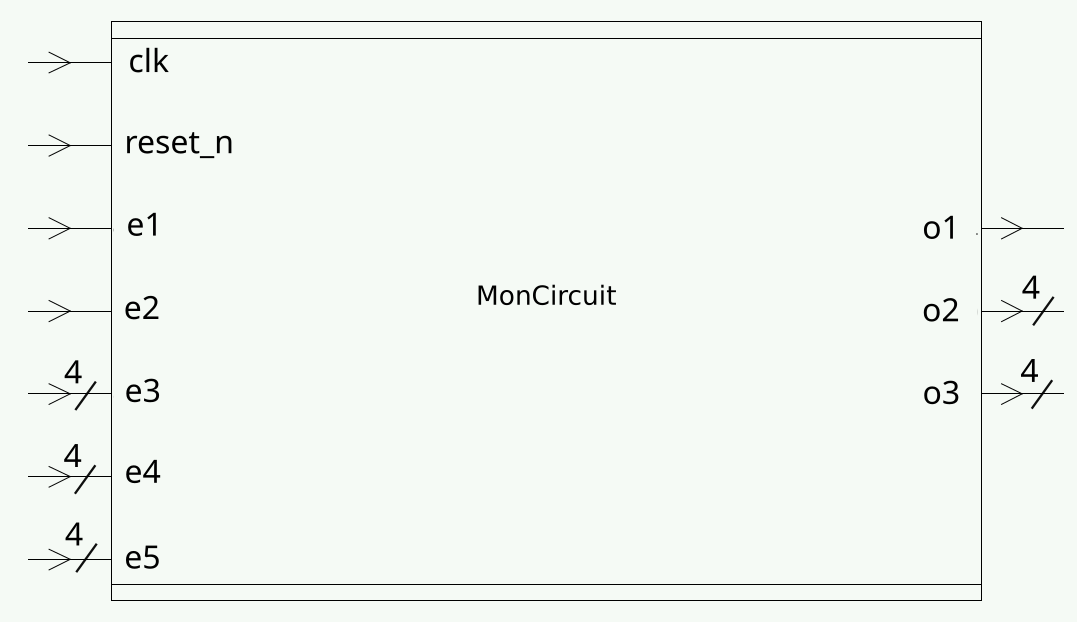
\includegraphics[width=8cm]{./images/entite.png}
    \captionof{figure}{Entity du composant MonCircuit}
    \label{moncircuit}
    \end{solbox}
    \fi

    \item Dessiner l'entité d'un demi-additionneur, puis le code VHDL de cette entité.

    \ifsolutions
    \begin{solbox}
    Voir la figure \ref{fig:ha}.
    \end{solbox}
    \fi

    \item Rappeler la constitution interne du demi-additionneur.

    \ifsolutions
    \begin{solbox}

      \begin{center}
        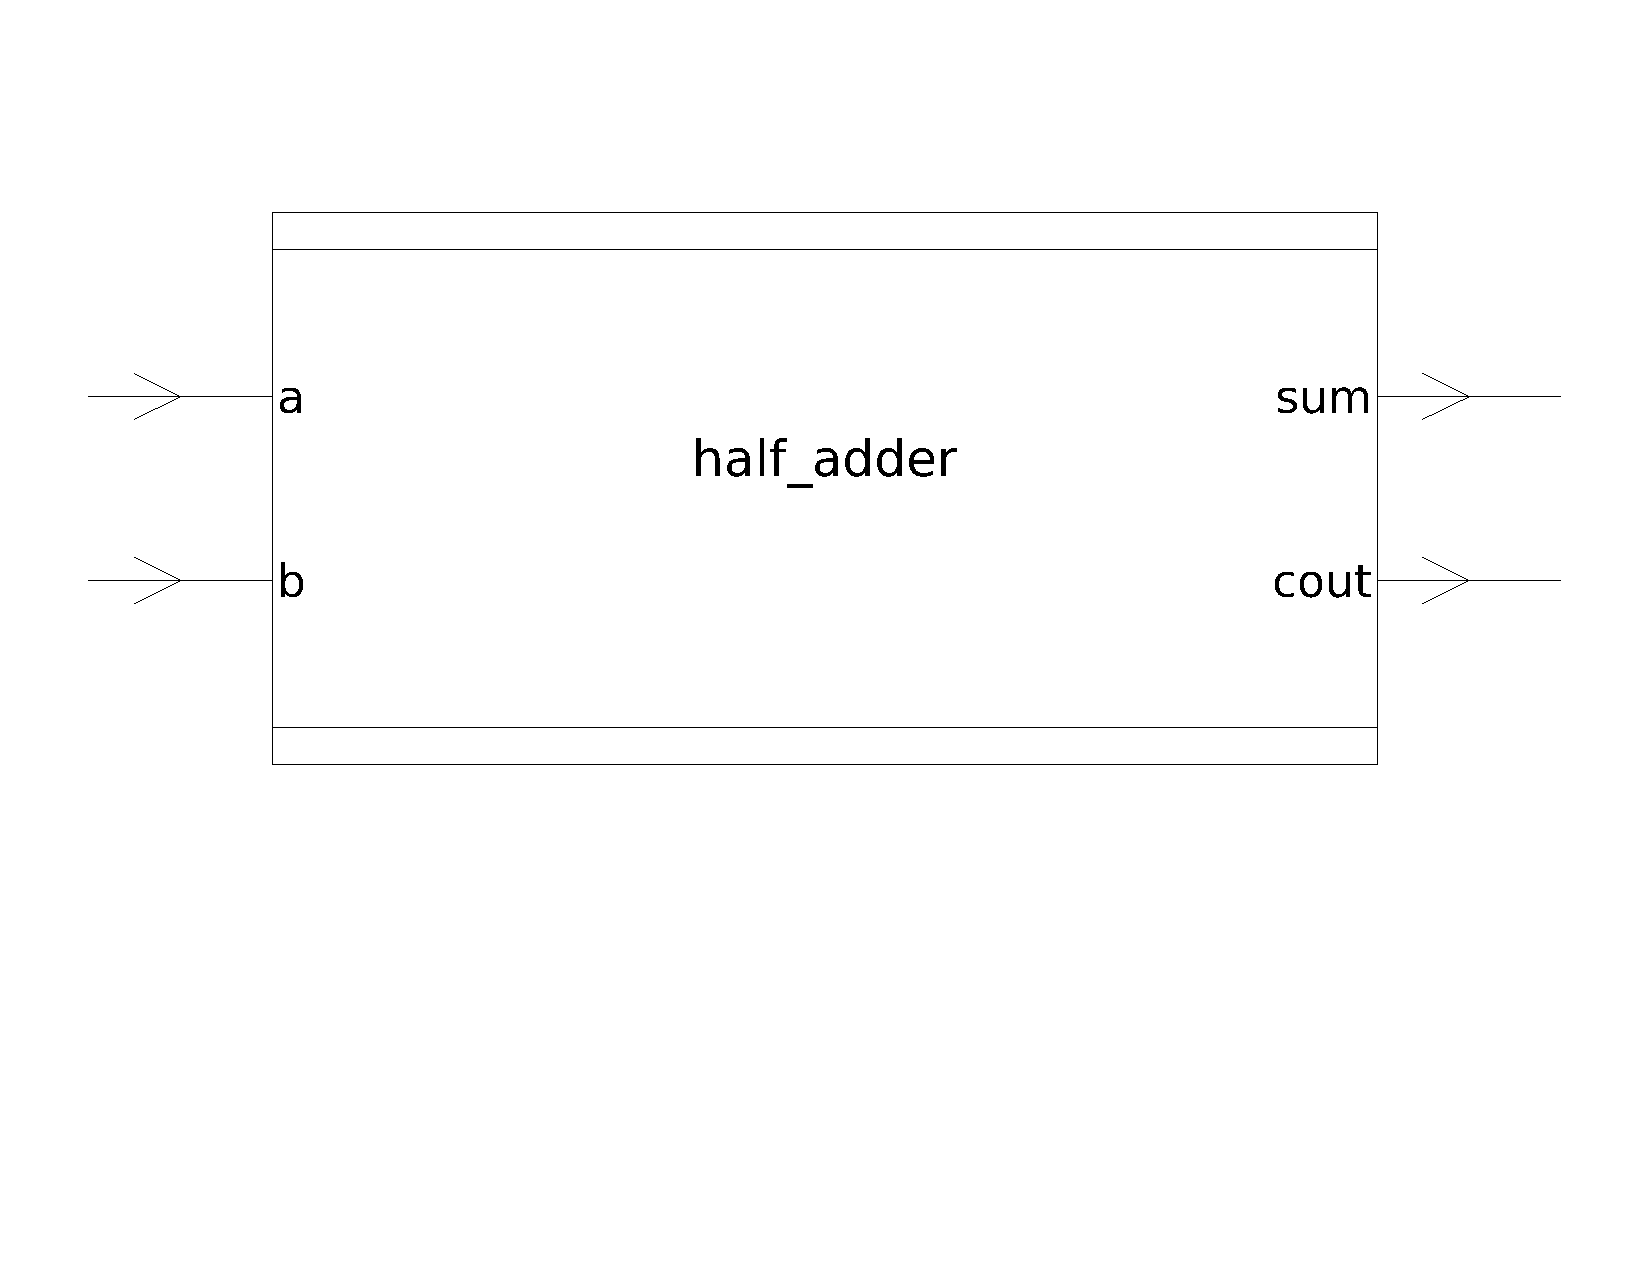
\includegraphics[width=6cm]{./codes/entity_half_adder.pdf}
        \hfill
        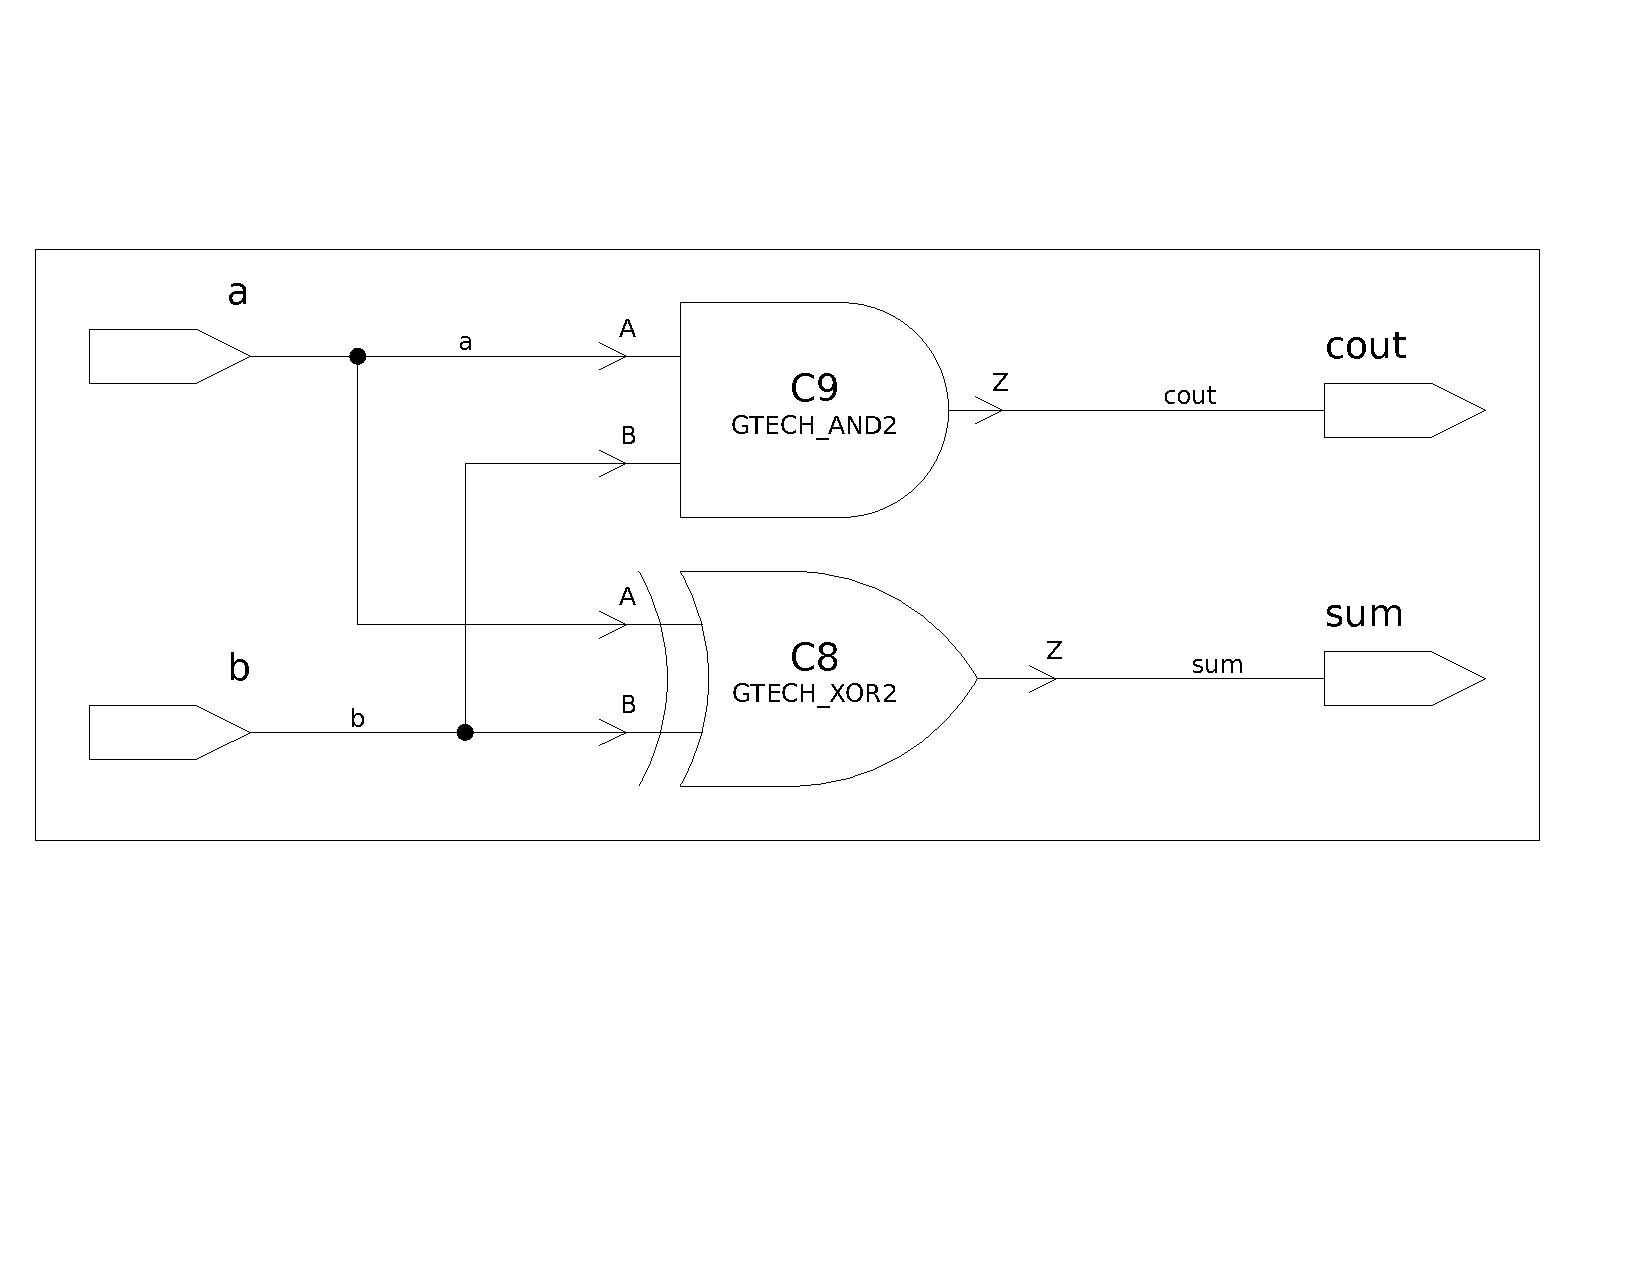
\includegraphics[width=7cm]{./codes/arch_half_adder.pdf}
        \captionof{figure}{Entity et architecture du demi-additionneur 1 bit}
        \label{fig:ha}
      \end{center}
    \end{solbox}
    \fi

    \item Coder l'architecture de ce demi-additionneur.

    \ifsolutions
    \begin{solbox}
    \lstinputlisting[language=VHDL]{./codes/half_adder.vhd}
    \end{solbox}
    \fi

    \item Dessinez la constitution interne d'un additionneur 1 bit complet, à partir du demi-additionneur.

    \ifsolutions
    \begin{solbox}
    \centering
    %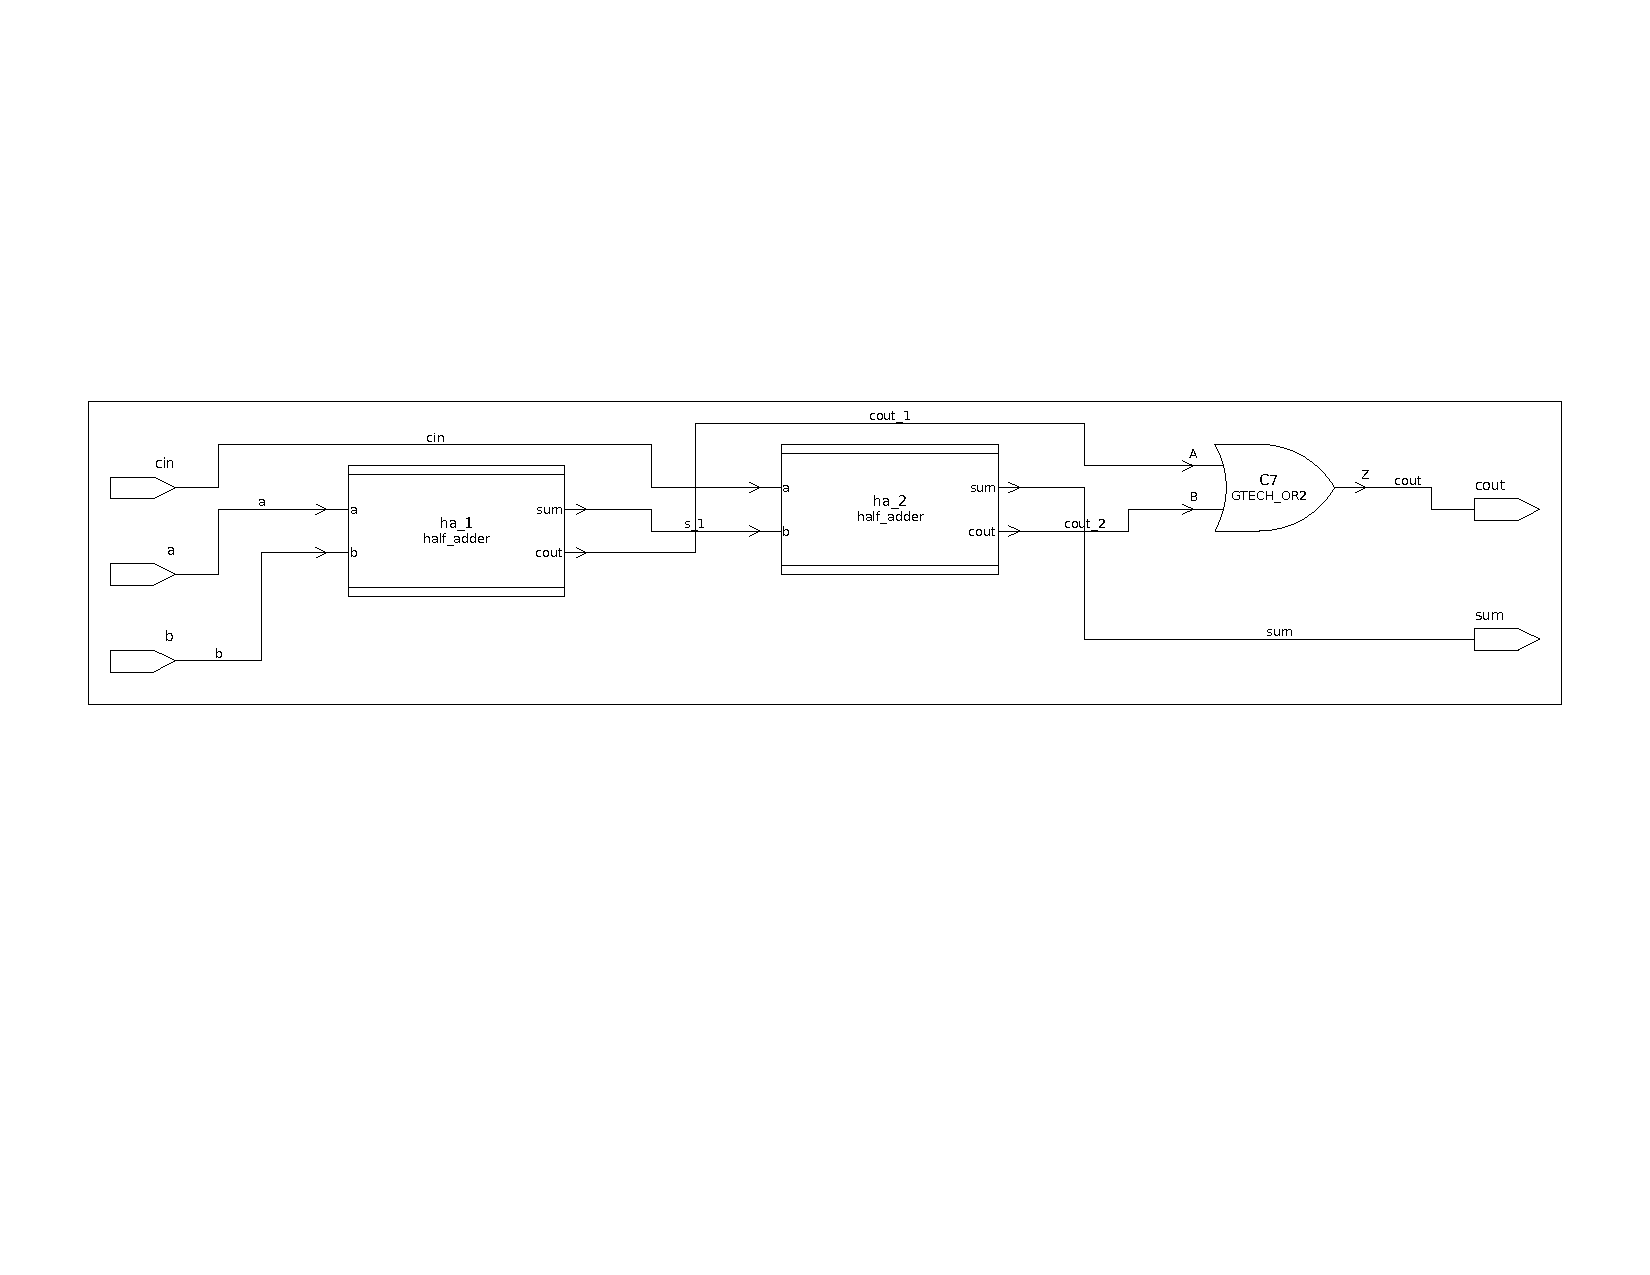
\includegraphics[width=13cm]{./codes/arch_full_adder.pdf}
    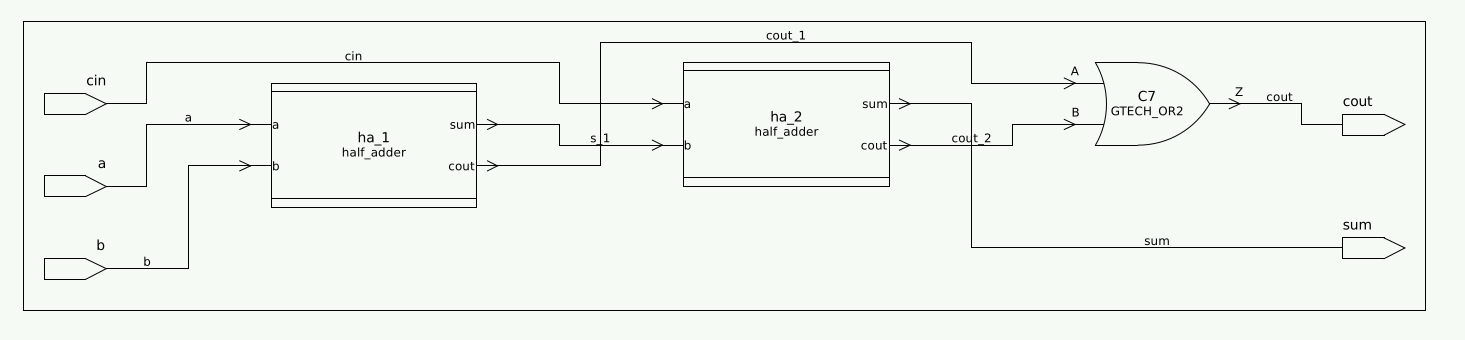
\includegraphics[width=13cm]{./images/fa_arch.png}
    \captionof{figure}{Architecture de l'additionneur 1 bit complet}
    \label{fig:full_adder}
    \end{solbox}
    \fi

    \item Coder en VHDL l'architecture de cet additionneur 1 bit.

    \ifsolutions
    \begin{solbox}
    \lstinputlisting[language=VHDL]{./codes/full_adder.vhd}
    \end{solbox}
    \fi

    \item Coder en VHDL l'entité et l'architecture d'un additionneur 8 bits.

    \ifsolutions
    \begin{solbox}
    \lstinputlisting[language=VHDL]{./codes/adder8b.vhd}
    \vspace{1em}
    \centering
    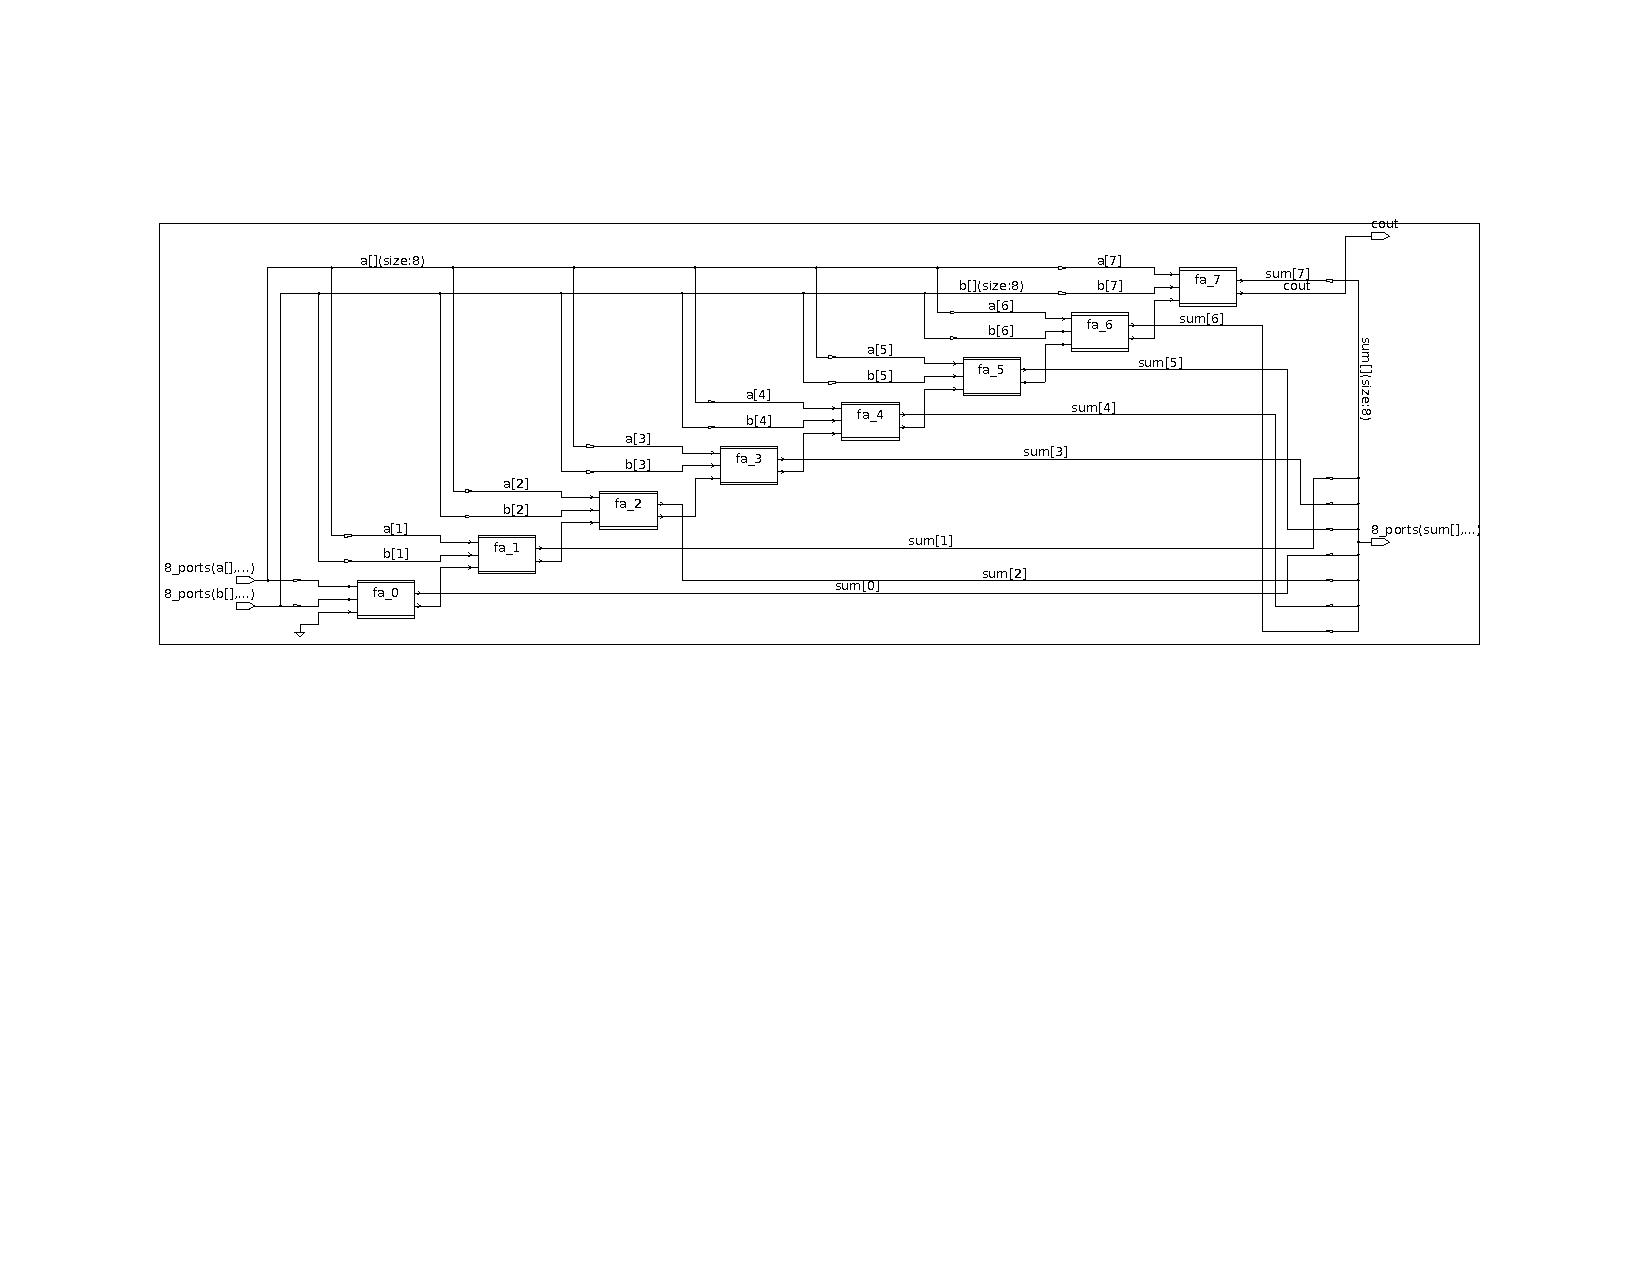
\includegraphics[width=15cm]{./codes/arch_adder8b.pdf}
    \captionof{figure}{Architecture de l'additionneur 8 bits}
    \label{fig:adder8b}
    \end{solbox}
    \fi
\end{enumerate}

\newpage

\section{Le banc de test (testbench)}

\begin{enumerate}
    \item Le testbench présente également une entité. Localisez cette entité. En quoi est-elle particulière ? Comment peut-on l'expliquer ?

    \ifsolutions
    \begin{solbox}
    Un tel banc de test possède une entité \textit{vide} : elle ne possède aucune entrée, ni sortie. C'est le laboratoire, portes closes.
    \end{solbox}
    \fi

    \item Un générateur d'horloge est contenu dans le banc de test. Combien de lignes sont nécessaires ? Dessinez le chronogramme de cette horloge.

    \ifsolutions
    \begin{solbox}
    Une seule ligne suffit. On inverse le signal tous les demi-périodes d'horloge, à l'aide d'une assignation conditionnée par un signal \texttt{running}, qui nous permettra de contrôler l'arrêt de la simulation.
    \end{solbox}
    \fi

    \item Comment notre banc de test provoque-t-il concrètement cet arrêt ?

    \ifsolutions
    \begin{solbox}
    Le signal \texttt{running} est affecté à \texttt{false} à la fin du processus de stimulation. Plus aucun événement n'est créé par le simulateur.
    \end{solbox}
    \fi

    \item Dessiner le chronogramme des stimuli.

    \ifsolutions
    \begin{solbox}
    \centering
    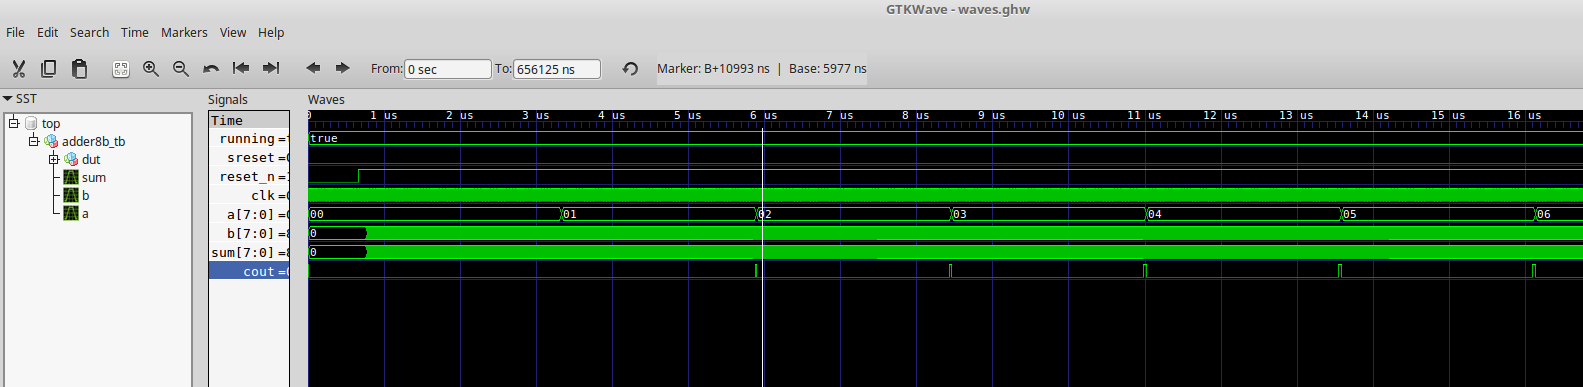
\includegraphics[width=14cm]{./codes/gtkwave_adder8b.png}
    \captionof{figure}{Chronogramme (overview)}
    \label{fig:chrono_overview}

    \vspace{1em}
    \centering
    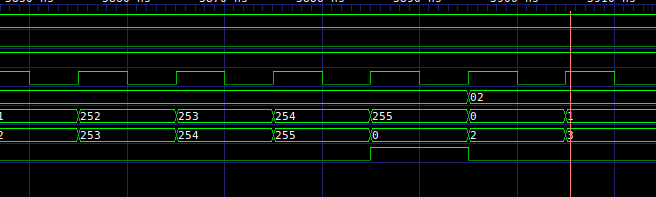
\includegraphics[width=14cm]{./codes/gtkwave_adder8b_1_255.png}
    \captionof{figure}{Chronogramme : cas de $1+255$}
    \label{fig:chrono_1_255}
    \end{solbox}
    \fi

    \item L'additionneur fonctionne-t-il avec des nombres signés ?

    \ifsolutions
    \begin{solbox}
    Oui ! En tous les cas, un test semble aller en ce sens ! Voir la figure \ref{fig:signed}.

    \vspace{1em}
    \centering
    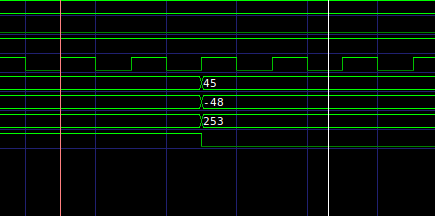
\includegraphics[width=14cm]{./codes/signed_values.png}
    \captionof{figure}{L'additionneur fonctionne pour les nombres signés}
    \label{fig:signed}
    \end{solbox}
    \fi
\end{enumerate}

\newpage

\section{Script de compilation}

\ifsolutions
\begin{solbox}
Script de compilation GHDL (donné sous Moodle) :

\begin{lstlisting}[style=bashstyle]
echo "=> cleaning..."
rm -rf waves.ghw *.o
echo "=> analyzing VHDL files..."
ghdl -a half_adder.vhd
ghdl -a full_adder.vhd
ghdl -a adder8b.vhd
ghdl -a adder8b_tb.vhd
echo "=> elaboration..."
ghdl -e adder8b_tb
echo "=> running simulation"
ghdl -r adder8b_tb --wave=waves.ghw
echo "=> starting waveform viewer"
gtkwave waves.ghw chrono.sav
\end{lstlisting}

\vspace{1em}
Testbench (donné sous Moodle) :

\lstinputlisting[language=VHDL]{./codes/adder8b_tb.vhd}
\end{solbox}
\fi

\section{Utilisation de \texttt{generate}}

\ifsolutions
\begin{solbox}
L'instruction \texttt{generate} permet de créer des instances de composants de manière itérative, ce qui est très utile pour structurer des designs réguliers comme un additionneur N bits.

\lstinputlisting[language=VHDL]{./codes/adder8b_generate.vhd}
\end{solbox}
\fi

\end{document}
